\begin{figure}
\centering
\captionsetup[subfigure]{font=footnotesize}
\begin{subfigure}{0.49\textwidth}
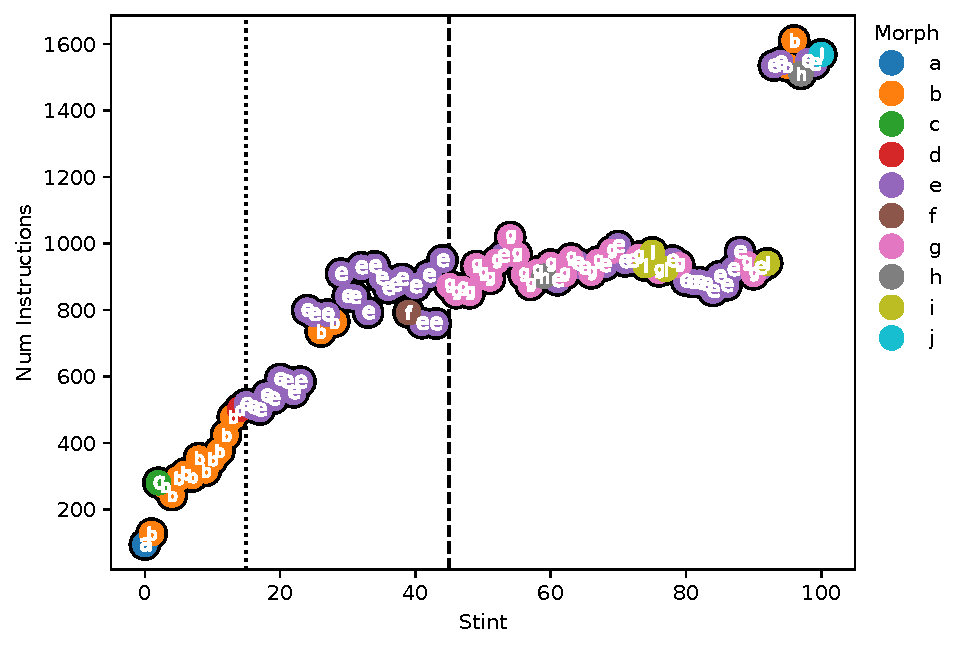
\includegraphics[width=\linewidth]{{submodule/dishtiny/binder/bucket=prq49/a=all_stints_all_series_profiles+endeavor=16/teeplots/bucket=prq49+cat=morph+endeavor=16+transform=filter-Series-16005+viz=letterscatter-vline+x=stint+y=num-instructions+ext=}}
\caption{instruction count}
\label{fig:instruction_count}
\end{subfigure}
\begin{subfigure}{0.49\textwidth}
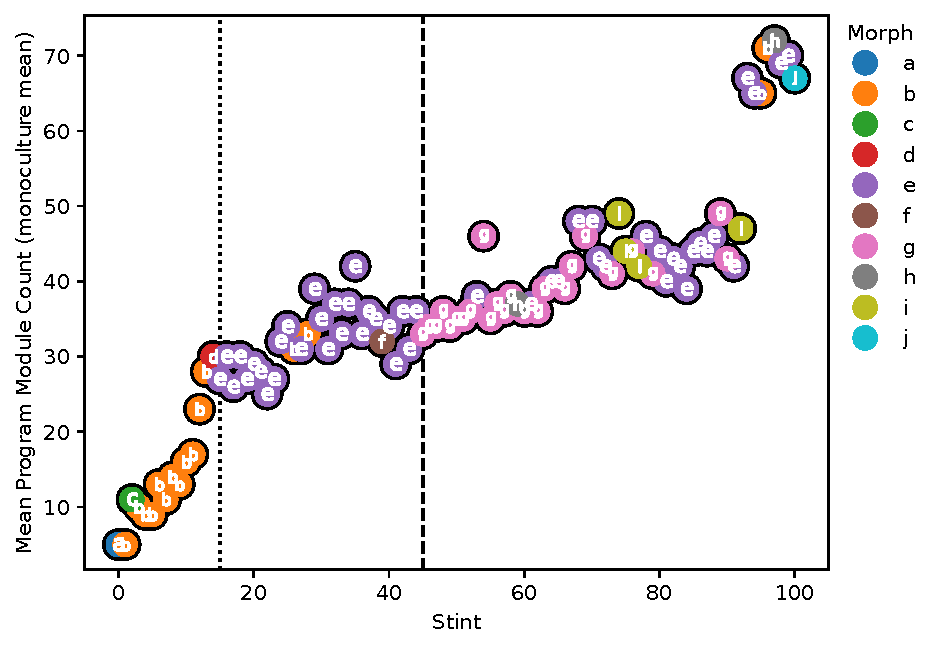
\includegraphics[width=\linewidth]{{submodule/dishtiny/binder/bucket=prq49/a=all_stints_all_series_profiles+endeavor=16/teeplots/bucket=prq49+cat=morph+endeavor=16+transform=filter-Series-16005+viz=letterscatter-vline+x=stint+y=mean-program-module-count-monoculture-mean+ext=}}
\caption{module count}
\label{fig:module_count}
\end{subfigure}
\begin{subfigure}{0.49\textwidth}
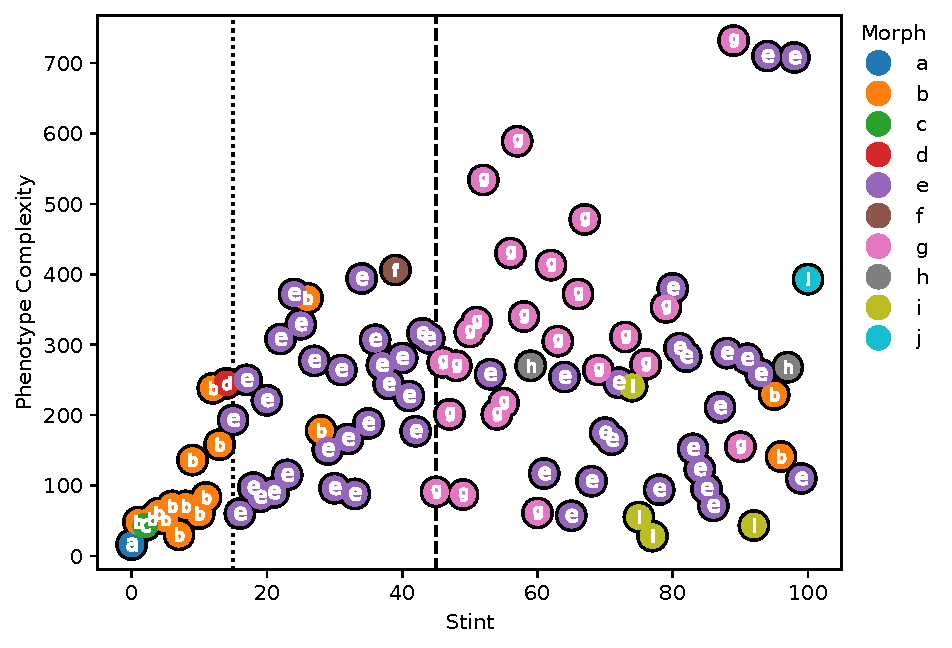
\includegraphics[width=\linewidth]{{plots/phenotype_complexity/bucket=prq49+cat=morph+endeavor=16+transform=filter-Series-16005+viz=letterscatter-vline+x=stint+y=phenotype-complexity+ext=}}
\caption{phenotype complexity}
\label{fig:phenotype_complexity}
\end{subfigure}

\caption{
\textbf{Genome content measures.}
\footnotesize
Instruction count is the total number of instructions present in the genome.
Module count is the number of tagged linear GP modules available for activation by signals from the environment, from other agents, or from within an agent.
Phenotype complexity is the number of genome sites that contribute to phenotype, measured as number sites remaining after phenotype-neutral nopout (Section \ref{sec:phenotype_neutral_nopout}).
This measure gives a sense of the number of ``active'' instructions that influence agents' behavior.
Color coding and letters correspond to qualitative morph codes described in Table \ref{tab:morph_descriptions}.
Dotted vertical line denotes emergence of morph $e$.
Dashed vertical line denotes emergence of morph $g$.
}
\label{fig:genome_size}

\end{figure}
